%%%%%%%%%%%%%%%%%%%%%%%%%%%%%%%%%%%%%%%%%%%%%%%%%%%%%%%%%%%%%%%%%%%%%%%%%%%%%%%%
%2345678901234567890123456789012345678901234567890123456789012345678901234567890
%        1         2         3         4         5         6         7         8

\documentclass[letterpaper,  10 pt,  conference]{ieeeconf}  % Comment this line out if you need a4paper

%\documentclass[a4paper,  10pt,  conference]{ieeeconf}      % Use this line for a4 paper

\IEEEoverridecommandlockouts                              % This command is only needed if 
                                                          % you want to use the \thanks command

\overrideIEEEmargins                                      % Needed to meet printer requirements. 

%In case you encounter the following error:
%Error 1010 The PDF file may be corrupt (unable to open PDF file) OR
%Error 1000 An error occurred while parsing a contents stream.  Unable to analyze the PDF file. 
%This is a known problem with pdfLaTeX conversion filter.  The file cannot be opened with acrobat reader
%Please use one of the alternatives below to circumvent this error by uncommenting one or the other
%\pdfobjcompresslevel=0
%\pdfminorversion=4

% See the \addtolength command later in the file to balance the column lengths
% on the last page of the document

% The following packages can be found on http:\\www. ctan. org
\usepackage{graphics} % for pdf,  bitmapped graphics files
\usepackage{epsfig} % for postscript graphics files
%\usepackage{mathptmx} % assumes new font selection scheme installed
%\usepackage{times} % assumes new font selection scheme installed
%\usepackage{amsmath} % assumes amsmath package installed
%\usepackage{amssymb}  % assumes amsmath package installed

\title{\LARGE \bf
Evaluation of Time Domain and Frequency Domain Classification Ability in Acceleration Tactile Signals
%加速度触覚信号における時間領域と周波数領域の分類能力の評価
%
%Research on comparison of usefulness in time domain and frequency domain of triaxial acceleration tactile signal
}


\author{Masahiro Koga$^{1}$,  Satoshi Saga$^{1}$,  Shotaro Agatsuma$^{2}$,  Junya Kurogi$^{1}$ and Tsuyoshi Usagawa$^{1}$ % <-this % stops a space
    \thanks{ $^{1}$Masahiro Koga, Satoshi Saga , Junya Kurogi and Tsuyoshi Usagawa,  Kumamoto University,  2-39-1,  Kurokami,  Chuo-ku,  Kumamoto Japan, 
    $^{2}$Shotaro Agatsuma,  University of Tsukuba,  1-1-1,  Tennodai,  Tsukuba,  Japan 
        %}% <-this % stops a space
    }
}


\begin{document}



\maketitle
\thispagestyle{empty}
\pagestyle{empty}


%%%%%%%%%%%%%%%%%%%%%%%%%%%%%%%%%%%%%%%%%%%%%%%%%%%%%%%%%%%%%%%%%%%%%%%%%%%%%%%%
\begin{abstract}
        Our previous studies have shown that CNN can classify time domain signals of acceleration tactile signals. 
        In this research,  we aim to 
        evaluate time domain and frequency domain classification ability,  dependency on input signal length in acceleration tactile signal through an experiment. 
        %guide future research,  investigate dependence depending on input signal length through simulation,  and investigate how the accuracy changes when the signal is converted to frequency domain using FFT. 

         The Experimental results show that the accuracy tends to increase as the data length increases in time domain signals.  In frequency domain signals, there was a problem that learning did not progress if the hyper parameters of the model were not changed. 
        Further this classification accuracy with advanced learning tended to stop at about 50 - 60\%. 
        In 1k Hz sampled both domain signals,  
        %ここをpossible と表現して良いものなのか
        it was found that classification is possible for 5 classes. 
        %Obviously over chance level in both the time domain and the frequency domain when using
        %in order to investigate the influence of the sampling frequency as well.  
        Also in this data,  it was found that the accuracy tends to improve in proportion to the data length. 
        %これまでの研究により、畳込みニューラルネットによって触覚加速度信号が分類できることがわかった。
        %本研究では、今後の研究の指針とすることを目的としシミュレーションを通して入力信号長に依る依存、及び信号をFFTを用いて周波数領域に変換した場合において精度がどのように変わるのかを調査する。
        %シミュレーションの結果、データ長が大きくなるにつれ精度も上がる傾向が見られた。FFTを用いてモデルのハイパラメータを入力以外に変更をくわえなかった場合
        %学習が進まないものがあった。学習が進んだものは50\%$\sim$60\%程度で学習が止まってしまう傾向が見られたが、分類が可能であることがわかった。サンプリング周波数の影響も調査するために5クラス分の1kサンプリングされたデータ
        %を用いた場合、時間領域、周波数領域ともに分類が可能であることがわかった。こちらのデータにおいてもデータ長に比例して精度が向上する傾向が見られることがわかった。
\end{abstract}


%%%%%%%%%%%%%%%%%%%%%%%%%%%%%%%%%%%%%%%%%%%%%%%%%%%%%%%%%%%%%%%%%%%%%%%%%%%%%%%%
\section{INTRODUCTION}
In recent years,  with the spread of tactile displays,  much research has been done on systems that collect information. The collected information is mainly applied to the output of tactile displays. 
In addition,  many attempts have been made to classify the collected information in order to provide an appropriate tactile presentation on the displays. 

In previous researches \cite{c1} \cite{c2},  they have developed a dedicated device that combines various sensors to collect tactile information. In these methods,  these researches collected
tactile information under a limited experimental environment,  in daily activities. To solve this problem our research group does not use integrated tactile sensors to detect tactile information.  
We have proposed a method to collect information easily \cite{c3}. 

In this proposed method,  the tactile information is limited to the acceleration information only.  
%and the tactile information is collected more easily than the equipment of the previous research by the wireless acceleration sensor \cite{c5}. 
Furthermore,  we have shown that it is possible to classify texture information by collecting accelerations of tactile motions on a desk and performing machine learning using a convolutional neural network (CNN).  
Machine learning using CNN has succeeded in classifying 30 types of data at approximately 90\%. 


In the previous research,  signal data was processed without processing,  that is,  classification was performed by inputting as a time series signal,  but it became necessary to investigate how the classification accuracy changes 
in different conditions or different processing procedures.  Therefore,  in this paper,  
we investigated classification ability between time domain and
frequency domain,  dependency on input signal length in
acceleration tactile signal through an experiment. 
%the dependence of data length and the change in accuracy when separation is performed using frequency domain signals.  
Furthermore,  we investigated how the accuracy changes with the sampling frequencies.  

%%%%%%引用%%%%%%

%近年、触覚ディスプレイの普及に伴い, 触覚情報を収集するシステムに関する研究が多く行われている. 収集された触覚情報は, 主に触覚ディスプレイの出力に応用されている. 
%また, 触覚ディスプレイにおいて適切な触覚提示を行うため, 収集された触覚情報を分類する試みも多く行われている. 先行研究においては, 触覚情報の収集と分類を両方行っている場合が多い. 
%
%
%これまでの先行研究 \cite{c1} \cite{c2} では, 様々なセンサを複合した専用の機器を開発して触覚情報の収集を行っている. これらの手法では限定的な実験環境下での触覚情報収集は可能であるが, 実験環境外, 
%例えば日常的な行動における触覚情報を収集することは難しい. この問題を解決するため, 我々の研究グループでは, 複雑な機器を用いずに触覚情報を容易に収集する手法を提案している \cite{c3}\cite{c4}. 
%
%この提案している手法では収集する触覚情報を加速度情報に限定し, 無線型加速度センサ\cite{c5}により, 先行研究の機器より手軽に触覚情報を収集する. 
%さらに, この手法により机上の触覚行動における加速度を収集し, 畳み込みニューラルネットワーク (CNN)を用いた機械学習を行うことで, 触覚動作の分類が可能であることを示してきた. これまでのところ, CNN を用いた機械学習により, 30 種類のデータを約 90\%で分類することに成功している. 
%
%%%%%%
%これまでの研究ではデータを無加工、つまり時系列信号として入力して分類を行っているが、条件や他の処理をした場合に分類
%精度がどのように変化するのかの調査が必要となった。そこで、本稿ではデータ長の依存、そして周波数領域信号で分離をした場合の
%精度の変化を調査を行った。さらに、サンプリング周波数でどのように精度が変化するのかを調査し、これらの依存関係についても調査を
%行った。
%
%

\section{EXPERIMENT SETUP}

The experiment conditions set for conducting the investigation will be described. 
In this Experiment,  data to be input to CNN is set as shown in the following table \ref{sim_set}. 
%今回、調査を行うために設定したシミュレーション条件について説明する。
%本シミュレーションではCNNに入力するデータを以下の表\ref{sim_set}のように設定した。

\begin{table}[htb]

    \begin{center}
        \caption{Experiment Settings}
        \begin{tabular}{|c|cc|cc|}\hline
             {Data type} & \multicolumn{4}{|c|}{Raw data,   FFT data}\\
             \hline
             {Sampling Freqency rate} & \multicolumn{2}{|c|}{330 Hz} & \multicolumn{2}{c|}{1k Hz}\\
             \hline
             {Data length}&128&256&128&256\\
             {}&512&800&512&1024\\

             \hline
        \end{tabular}
    \label{sim_set}
    \end{center}

\end{table}
%``''

This time,  we name data obtained from the sensor module ``raw data'',  and a Fast Fourier Transform (FFT) amplitude spectrogram of raw data ``FFT data''. 







Regarding model input,  3ch with $x,  y$, and $z$ axes data obtained from the acceleration sensor is used as input,  and the classification accuracy in the case of changing the input data length is evaluated. 
The NN used this time is a model based on the Convolutional Neural Network (CNN).  This model is an improvement based on VGG 16 \cite{c6} and uses parameters adapted to input data. 
A schematic diagram of the basic model of this CNN is shown in the following Fig. \ref{model_arch}. 

% 今回、センサモジュールから得られたデータを生データと呼び、生データのFFT振幅スペクトログラムをFFTデータと呼ぶ。
%
%モデル入力に関して、センサから得られたx、y、zデータを入力とした3chを入力とし、入力データ長を変化させた場合の分類精度を評価する。
%今回使用したNNはConvolutional Neural Network(以下CNN) をベースとしたモデルとなっている。このモデルはVGG16\cite{c6}をベースに改良したもので、更に入力データに
%適応させたパラメータを使用する。
%今回のCNNの基礎モデルの概略図を以下の図\ref{model_arch}に示す。

\begin{figure}[thpb]
    \centering
    %\framebox{\parbox{3in}{本研究ではこのモデルを基本モデルとし、入力サイズ、畳み込み層の出力特徴数、畳み込み層の層数を調整し入力データに対する学習を進める。
    %}}




%%./../

    \includegraphics[scale=0.30]{./../figs/fig1_arch_with_sub.eps}
    \caption{Basic CNN model in this research. In this research,  this model is used as a basic model,  and the input size,  the number of output features of the convolutional layer,  
    and the number of layers of the convolutional layer are adjusted to advance learning for the input data. 
    %本研究ではこのモデルを基本モデルとし、入力サイズ、畳み込み層の出力特徴数、畳み込み層の層数を調整し入力データに対する学習を進める。
    }
    \label{model_arch}
 \end{figure}

 The additional operation of bias and the activation processing by the LeakyReLU function are performed for each block in Fig. \ref{model_arch}. 
 Moreover,  the softmax function was used for the activation function of the output layer,  and the loss function used the cross entropy error.  We used Adam Optimizer \cite{c7} as the optimization algorithm 
 for learning,  repeated learning until the training accuracy converged,  and then evaluated the accuracy of the test data. \\

%図\ref{model_arch}中の各ブロックごとにバイアスの加算演算、LeakyRelu関数による活性化処理を行っている。また、出力層の活性化関数にはsoftmax関数を用い、損失関数は
%クロスエントロピー誤差を用いた。学習の際の最適化アルゴリズムにはAdam\cite{c7}を用い、訓練精度が収束するまで学習を繰り返しおこなった後、テスト用データにおける精度評価を行った。




\textbf{HOW TO EXPERIMENT}


In this experiment,  the data set is divided into 
$training: test = 8: 2$
and the CNN model is trained using the training data set. 
Using training data,  measure the accuracy of the learned model with test data. The batch size of test input is 32 and accuracy is given for each batch.  
The test is performed 10 times,  and the maximum,  minimum and average accuracy among them are calculated to evaluate the model. 

%今回行うシミュレーションでは、データセットをトレーニング:テスト=8:2となるように分割し、トレーニングデータセットを用いてCNNモデルを学習させていく。
%トレーニングデータにより学習済みモデルをテストデータで精度を計測する。テスト入力のバッチサイズは32として、バッチごとに精度を出す。テストを10回行い、
%そのうちの最大、最小、平均精度を算出しモデルの評価を行う。

\section{%結果 
Result of Experiment}
\textbf{Results of 330 Hz sampling data}\\
The following Fig. \ref{330_ave_stddev} shows the accuracy when changing the input data length in raw data and FFT data.  As data used at this time,  32 out of 300 prepared 
test data groups were randomly used. The accuracy of the minimum-maximum value when this is repeated 10 times is shown. \\
%以下の表\ref{acc_compare1}に生データ及びFFTデータにおいて入力データ長を変化させた時の精度を示す。この時使用したデータは、300個用意したテストデータ群のうち、ランダムに32個を使用した。これを10回繰り返したときの最小-最大値の精度を示す。\\


\begin{figure}[thpb]
    \centering
    %\framebox{\parbox{3in}{本研究ではこのモデルを基本モデルとし、入力サイズ、畳み込み層の出力特徴数、畳み込み層の層数を調整し入力データに対する学習を進める。
    %}}



%./graph1.png
    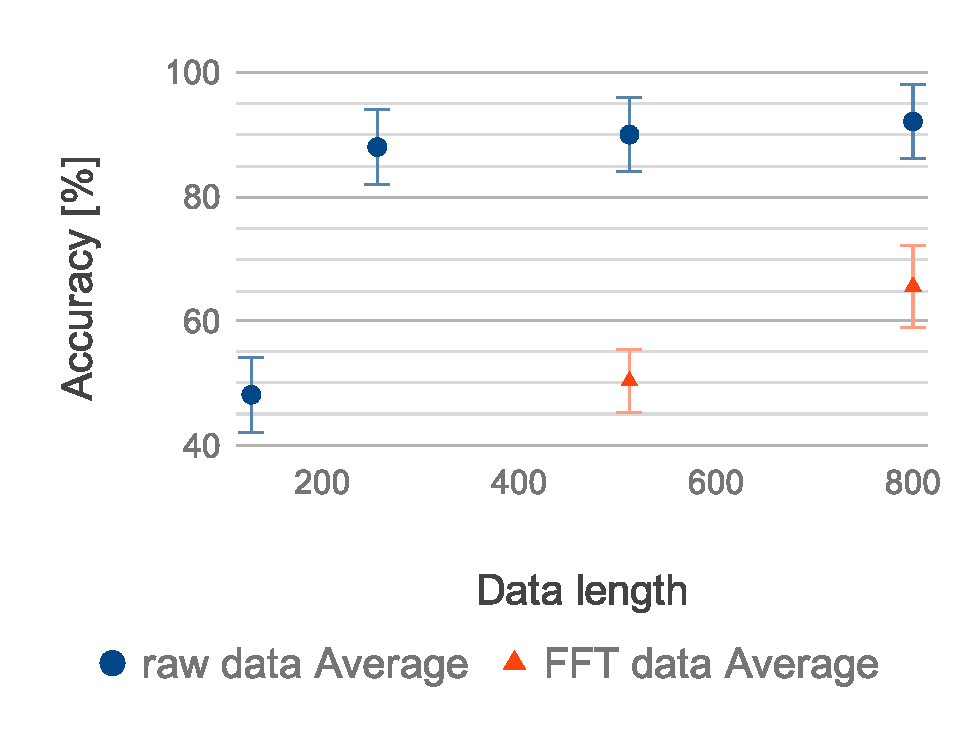
\includegraphics[scale=0.53]{./../figs/chart330.eps}
    \caption{
        Test accuracy average and standard deviation of 330 Hz data
    %本研究ではこのモデルを基本モデルとし、入力サイズ、畳み込み層の出力特徴数、畳み込み層の層数を調整し入力データに対する学習を進める。
    }
    \label{330_ave_stddev}
 \end{figure}

%\begin{table}[h]
%    \begin{center}
%        
%        \begin{tabular}{|c|c|c|}
%            \hline
%            \bf{data length}& \bf{raw data} & \bf{FFT data} \\ \hline
%             128 & 48.2 - 15.2 & Training impossible \\ \hline
%             256 & 88.0 - 4.4 & Training impossible \\ \hline
%             512 & 90.0 - 6.3 & 50.0 - 4.8 \\ \hline
%             800 & 92.1 - 3.4& 65.6 - 1.96 \\ \hline
%            \end{tabular}
%        
%    \caption{%330 Hz, 生データ及びFFTデータの入力データ長を変化させたときのテストデータに対するモデルの識別精度の比較
%    Comparison of model identification accuracy to test data when input data length of 330  Hz,  raw data and FFT data is changed.Each value in the table represents the accuracy [\%] of minimum-maximum-average.}
%    \label{acc_compare1}
%    \end{center}
%\end{table}

%    \begin{table}[h]
%        \begin{center}
%            
%            \begin{tabular}{|c|c|c|}
%                \hline
%                \bf{data length}& \bf{raw data} & \bf{FFT data} \\ \hline
%                128 & 31.3 - 65.6 - 48.2 & Training impossible \\ \hline
%                 256 & 81.3 - 90.6 - 88.8 & Training impossible \\ \hline
%                 512 & 84.3 - 96.8 - 90.0 & 43.8 - 53.1 - 50.4 \\ \hline
%                 800 & 88.1 - 96.8 - 92.1 & 53.1- 68.8 - 65.6 \\ \hline
%                \end{tabular}
%            
%        \caption{%330 Hz, 生データ及びFFTデータの入力データ長を変化させたときのテストデータに対するモデルの識別精度の比較
%        Comparison of model identification accuracy to test data when input data length of 330  Hz,  raw data and FFT data is changed.Each value in the table represents the accuracy [\%] of minimum-maximum-average.}
%        \label{acc_compare1}
%        \end{center}
%    \end{table}

%    次に以下の表\ref{acc_compare2}にFFTのパワースペクトログラムデータにおいて入力データ長を変化させた時の精度を示す。\\

%    \begin{table}[h]
%        \begin{center}
%            
%            \begin{tabular}{|c|c|}
%                \hline
%                \bf{data length}& \bf{test accuracy Min-Max-Ave \%}\\ \hline
%                 128 & 学習不可 -  -\\ \hline
%                 256 & 学習不可 -  -\\ \hline
%                 512 & 43.8 - 53.1 - 50.4\\ \hline
%                 800 &  53.1- 68.8 - 65.6\\ \hline
%                \end{tabular}
%            
%        \caption{330 Hz, FFTデータの入力データ長を変化させたときのテストデータに対するモデルの識別精度の比較}
%        \label{acc_compare2}
%        \end{center}
%    \end{table}
\textbf{Results of 1k Hz sampling data}\\

The following Fig. \ref{1k_ave_stddev} shows the accuracy when 1k Hz sampling raw data and FFT data are changed in the input data length. As data used at this time,  32 out of 120 prepared test data groups were randomly used. The accuracy of the minimum-maximum-average is shown when this is repeated 10 times. \\
    %以下の表\ref{acc_compare3}に1k サンプリングの生データ及びFFTデータにおいて入力データ長を変化させた時の精度を示す。この時使用したデータは、120個用意したテストデータ群のうちランダムに32個を使用した。これを10回繰り返したときの最小-最大値-平均の精度を示す。\\

    \begin{figure}[thpb]
        \centering
        %\framebox{\parbox{3in}{本研究ではこのモデルを基本モデルとし、入力サイズ、畳み込み層の出力特徴数、畳み込み層の層数を調整し入力データに対する学習を進める。
        %}}



        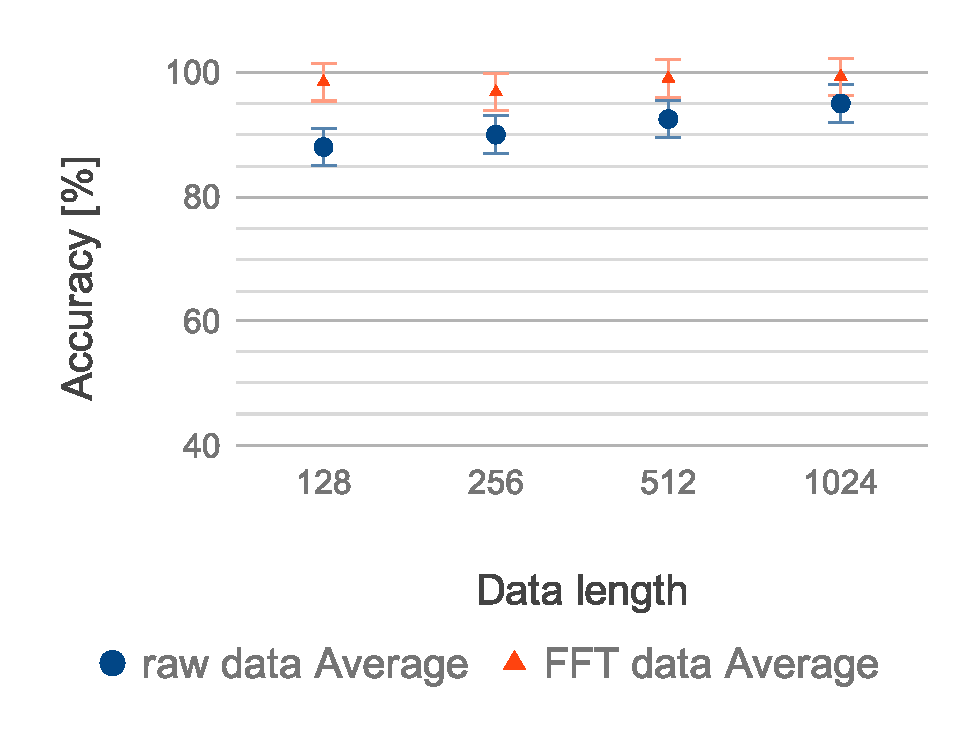
\includegraphics[scale=0.53]{./../figs/chart1k.eps}
        \caption{
            Test accuracy average and standard deviation of 1k Hz data 
        %本研究ではこのモデルを基本モデルとし、入力サイズ、畳み込み層の出力特徴数、畳み込み層の層数を調整し入力データに対する学習を進める。
        }
        \label{1k_ave_stddev}
     \end{figure}    

%    \begin{table}[h]
%        \begin{center}
%        
%            \begin{tabular}{|c|c|c|}
%                \hline
%                \bf{data length}& \bf{raw data} & \bf{FFT data} \\ \hline
%                128 &  88.8 - 5.3& 98.4 - 1.6\\ \hline
%                256 &  90.0 - 7.8& 96.8 - 1.9\\ \hline
%                512 &  92.5 - 6.4& 99.0 - 1.7\\ \hline
%                1024 &  95.0 - 4.1& 99.3 - 1.8\\ \hline
%            \end{tabular}
            
%            \caption{Comparison of model identification accuracy to test data when input data length of 1k  Hz,  raw data and FFT data is changed.Each value in the table represents the accuracy [\%] of minimum-maximum-average.}
%            \label{acc_compare3}
%    \end{center}
%\end{table}

%\textbf{1k Hz sampling data}\\
%    The following table \ref{acc_compare3} shows the accuracy when 1k sampling raw data and FFT data are changed in input data length. As data used at this time,  32 out of 120 prepared test data groups were randomly used. The accuracy of the minimum-maximum-average is shown when this is repeated 10 times. \\
%        %以下の表\ref{acc_compare3}に1k サンプリングの生データ及びFFTデータにおいて入力データ長を変化させた時の精度を示す。この時使用したデータは、120個用意したテストデータ群のうちランダムに32個を使用した。これを10回繰り返したときの最小-最大値-平均の精度を示す。\\
%
%
%        \begin{table}[h]
%            \begin{center}
%            
%                \begin{tabular}{|c|c|c|}
%                    \hline
%                    \bf{data length}& \bf{raw data} & \bf{FFT data} \\ \hline
%                    128 &  87.5- 96.8 - 88.8 & 96.8 - 100 - 98.4 \\ \hline
%                    256 &  81.3 - 96.8 - 90.0 & 93.8 - 100 - 96.8 \\ \hline
%                    512 &  81.3 -  96.8 - 92.5 & 96.8 - 100 - 99.0 \\ \hline
%                   1024 &  92.1 -  100 - 95.0 & 96.8 - 100 - 99.3 \\ \hline
%               \end{tabular}               
%                \caption{Comparison of model identification accuracy to test data when input data length of 1k  Hz,  raw data and FFT data is changed.Each value in the table represents the accuracy [\%] of minimum-maximum-average.}
%                \label{acc_compare3}
%        \end{center}
%    \end{table}

    %次に以下の表\ref{acc_compare4}にFFTのパワースペクトログラムデータにおいて入力データ長を変化させた時の精度を示す。\\

    %\begin{table}[h]
    %    \begin{center}
    %        
    %        \begin{tabular}{|c|c|}
    %            \hline
    %            \bf{data length}& \bf{test accuracy Min-Max-Ave \%}\\ \hline
    %             128 & 96.8 - 100 - 98.4\\ \hline
    %             256 & 93.8 - 100 - 96.8\\ \hline
    %             512 & 96.8 - 100 - 99.0\\ \hline
    %             1024 & 96.8 - 100 - 99.3\\ \hline
    %            \end{tabular}
    %        
    %    \caption{1k Hz, FFTデータの入力データ長を変化させたときのテストデータに対するモデルの識別精度の比較}
    %    \label{acc_compare4}
    %    \end{center}
    %\end{table}

\section{%考察
CONSIDERATION}
This experimental result shows that it can be seen that features can be found from the time domain and the frequency domain since the chance level is clearly exceeded in any case.
%data can be classified regardless of raw data 
In addition,  the accuracy tended to be monotonically increasing to the data length.  
This tendency was observed in both time domain data and frequency domain data. 
In the classification of 330 Hz data,  when the data length is 128,  the accuracy is low compared to other data lengths,  and the small amount of information suggests 


that CNN may not have been able to capture features.  However,  further problems were found in this survey,  such as the setting of hyper-parameters and issues with a different number of classes of 1k Hz data. 
%今回の実験の結果よりどの場合においてもチャンスレベルを明らかに超えているので、時間領域と周波数領域から特徴を見つけることができていることがわかる。
%
%330 Hzデータの分類では、データ長が128の時はその他のデータ長に比べて大きく精度が低いことから、情報量の少なさから、CNNが特徴を捉えることができていない可能性が示唆される。
%しかし、CNNパラメータの設定や、1k Hzデータのクラス数が違う問題など、今回の調査からさらなる課題が見つかった。




\section{CONCLUTION AND FUTURE WORK}

In this experiment,  the number of classes are 30 classes for 330 Hz data and 5 classes 1k Hz data. Thus , the effect of the sampling frequency was not correctly evaluated.  
However,  when the time domain data and the frequency domain data are compared at the same sampling frequency,  the frequency domain data is accurate,  so that the frequency 
resolution may be increased by the increase of the sampling frequency,  and the signal feature may be easily grasped. As a future work,  we plan to investigate the control 
effect of hyperparameters of CNN model since there is a possibility that the accuracy may change by optimization. 
%今回のシミュレーションでは330 Hzデータと1k Hzデータにおいてクラス数が 30クラスと5クラスとなっており、サンプリング周波数の影響は真にはわからなかった。しかし、
%同じサンプリング周波数において時間領域データと周波数領域データを比較したときに周波数領域データが精度が良かったことから、サンプリング周波数が上がることにより
%周波数解像度が上がり、信号の特徴を捉えやすくなる可能性が示唆された。また、CNNパラメータを固定せず、最適化を行うことにより精度が変わる可能性もあるため、今後は
%それらについての調査もやっていこうと思う。

%%今後はCNNパラメータの最適値や1k Hzデータのクラス数の補強などをし、各種法の有用性を調査しなければならないだろう。


%\section{まとめ Conclusion}
%本稿により生データを使用することの有用性を示すことができ、
%またデータ長に関する指標の一つとすることができたのではないかと思う。
%今回はFFTの振幅信号のみを用いたが、他にも様々な手法の信号処理技術があり、
%今後の研究では更に他の処理を検討する必要も考えられる。
%また、1k Hzのデータに関してはクラス数も少なく真にサンプリング周波数を上げる
%有用性が示すことができていないため、こちらのデータもさらに増強することで
%サンプリング周波数との関係も調査する必要が出てきた。



\addtolength{\textheight}{-12cm}  % This command serves to balance the column lengths
                                  % on the last page of the document manually. It shortens
                                  % the textheight of the last page by a suitable amount.
                                  % This command does not take effect until the next page
                                  % so it should come on the page before the last. Make
                                  % sure that you do not shorten the textheight too much.

%%%%%%%%%%%%%%%%%%%%%%%%%%%%%%%%%%%%%%%%%%%%%%%%%%%%%%%%%%%%%%%%%%%%%%%%%%%%%%%%



%%%%%%%%%%%%%%%%%%%%%%%%%%%%%%%%%%%%%%%%%%%%%%%%%%%%%%%%%%%%%%%%%%%%%%%%%%%%%%%%



%%%%%%%%%%%%%%%%%%%%%%%%%%%%%%%%%%%%%%%%%%%%%%%%%%%%%%%%%%%%%%%%%%%%%%%%%%%%%%%%

%\section*{APPENDIX}

%\section*{ACKNOWLEDGMENT}



%%%%%%%%%%%%%%%%%%%%%%%%%%%%%%%%%%%%%%%%%%%%%%%%%%%%%%%%%%%%%%%%%%%%%%%%%%%%%%%%



\begin{thebibliography}{99}

    \bibitem{c1} Arsen Abdulali and Seokhee Jeon. Data-Driven Modeling of Anisotropic Haptic Textures: Data Segmentation and Interpolation. In Haptics: Perception,  Devices,  Control, and Applications: 10th International Conference,  Euro
    Haptics 2016,  London,  UK,  pp. 228 - 239. Springer International Publishing,  2016.

    \bibitem{c2}Matti Strese,  Yannik Boeck,  and Eckehard Steinbach. Content-based Surface Material Retrieval. In 2017 IEEE World Haptics Conference (WHC),  F ̈urstenfeldbruck (Munich),  Germany,  pp. 352 - 357. IEEE,  2017.
    
    \bibitem{c3}Shotaro Agatsuma and Shinji Nakagawa and Tomoyoshi Ono and Satoshi Saga and Simona Vasilache and Shin Takahashi. Classification Method of Rubbing Haptic Information Using Convolutional Neural Network. In Proceedings of
     International Conference,  HCI International 2018,  Palermo , Italy,  pp.159 - 167. IEEE, 2018
   
    %\bibitem{c3}嵯峨智,  中川真史,  小野智義,  潘振雷,  張嘉袁. Zigbee を利用した日常の触覚情報収集. 電気学会研究会資料 (知覚情報研究会・力触覚提示デバイス),  Vol. 2017,  No. 52,  pp. 11–14,  2017.
    
    %\bibitem{c4}我妻正太郎,  中川真史,  小野智義,  嵯峨智,  高橋伸. Zigbee マイコンによる触覚情報収集と深層学習による分類手法. 第18 回計測自動制御学会システムインテグレーション部門講演会予稿集,  pp. 467–471. 計測自動制御学会,  2017.
 
    \bibitem{c5} Mono Wireless Inc. TWE-Lite-2525A. (https://mono-wireless.com/jp/products/TWE-Lite-2525A).

    \bibitem{c6} Karen Simonyan and Andrew Zisserman. Very Deep Convolutional Networks for Large-Scale Image Recognition. arXiv:1409. 1556,  2014. 

    \bibitem{c7}Diederik Kingma and Jimmy Ba. Adam: A method for stochastic optimization. arXiv preprint arXiv:1412. 6980, 2014. 
\end{thebibliography}


\end{document}
